%\documentclass[12pt]{scrreprt}
\documentclass[12pt]{report} 

% language may be romanian or english (default is english)
% type may be bachelor or master (default is bachelor)
\usepackage[language=eng, type=bachelor]{style}

%\geometry{a4paper,top=2.5cm,left=3cm,right=2.5cm,bottom=2.5cm}
%in style
%controlling the appearance of your headers and footers
\usepackage{fancyhdr}
\pagestyle{fancy}
\lhead{}
\chead{}
\renewcommand{\headrulewidth}{0.2pt}
\renewcommand{\footrulewidth}{0.2pt}

\begin{document}

\specialization{COMPUTER SCIENCE}	
\title{Integrating NFC data retrieval in Android mobile applications}					   
\author{Fodor George-David}											
\supervisor{Phd. Student Țirban Ionuț-Paul\newline
Phd. Coroiu Adriana Mihaela}				
				
\maketitle


\newpage
\thispagestyle{empty}
\mbox{}
\newpage
\pagenumbering{roman} 

\cleardoublepage
ABSTRACT
\vspace{0.5cm}	
\hrule
\vspace{0.5cm}	
%\cleardoublepage

The main purpose of our paper, "Integrating NFC data retrieval in Android mobile applications", is to give an example of how the NFC could be used in different domains in order to retrieve information while providing a new layer of privacy for the users. A second goal is to serve a solution for the medical system that can be easily implemented in order to get rid of the paper medical reports and take full advantage of the Electronic Medical Record (EMR) systems.

The first part of our paper, chapter two, presents the current situation and the solution we are proposing.

Part two, chapters three and four, talk about the architecture and system requirements for the application we are aiming to develop in order reach the goal stated in the last section of chapter two.

The final part, chapters five and six, present our results and the improvements we consider that should be mentioned.

\tableofcontents


\newpage
\pagenumbering{arabic}

\chapter{Introduction}
\label{intro}

\par With our application, "Medical Reports", we have tried to look into how we could help improve the retrieval of patients' information from a remote Electronic Medical Record (EMR) system by incorporating the usage of NFC (Near-Field Communication) tags in the patients' bracelets.

The current solutions for EMR systems do not provide an easy and privacy supportive way of retrieving data about the patients. The most used solution is printing medical reports on paper and using that in order to keep track of the state of the patient. Some of that data might never be recorded, which is also a problem, but the bigger issue is the fact that those files are usually left somewhere in the proximity of the patient, which present a privacy infringement as information can easily be extracted by unauthorized humans.

The second chapter addresses multiple topics regarding the NFC technology and its uses and the privacy. In the first section of chapter 2 we will talk about the NFC technology, what it is and some of its applications. The second section will talk about the NFC technology in Android, how it is currently being used and what the possibilities are. The third section presents the usages of the NFC in specific domains, among which is also the health care system. In section 4 we will talk about some alternatives to NFC in the Health Tech space. Section 5 of this chapter presents the privacy concerns regarding our society in different domains, among which are the health care system and the usage of NFC. Section 6 talks about our proposed solution and what we aim to achieve.

The third chapter presents the architecture that has been implemented in our application as well as a reasoning behind the choices we have made regarding the server application.

In chapter 4 we will present the system requirements in order to run the server application as well as the system requirements for the android application.

In the fifth chapter we created a user manual for the application we have managed to create and we explained some of the logic behind.

The sixth chapter presents what our view on the future of "Medical Reports" application and the improvements that we really think will be necessary in order for this to be a proper solution for an actual implementation in the Health Tech space.

The last chapter, number 7, contains our conclusions about the subject and what we managed to achieve.
%\addcontentsline{toc}{chapter}{Introduction}

\chapter{NFC Usage In Health Tech, Android NFC \& Privacy}
\label{chap:ch2}

\section{NFC Technology}
\label{sec:ch2sec1}

\par Near Field Communication (NFC) is a standards-based short-range wireless connectivity technology that makes life easier and more convenient for consumers around the world by making it simpler to make transactions, exchange digital content, and connect electronic devices with a touch. NFC is compatible with hundreds of millions of contactless cards and readers already deployed worldwide. \cite{whatIsNFC}

NFC is distinct from far field RF communication that is used in personal area and longer-range wireless networks. NFC relies on inductive coupling between transmitting and receiving devices. The communication occurs between two compatible devices within few centimeters with 13.56 MHz operating frequency. \cite{coskun2013survey}

We have to remember that there are three major devices in NFC: NFC enabled mobile phones, NFC readers and NFC tags. NFC communication occurs between two NFC devices with some valid combinations. For example a mobile phone may communicate with a NFC reader. \cite{coskun2011near}

As the communication method of NFC is a very close range one it is very common that the user will actually touch their phone to the NFC reading device or NFC tag. That's why this process might also be known as the touching paradigm. The user must always be aware in order to perform near field communication, as the user needs to actively "touch" the other communication device, being it either a NFC reader, a tag, or another NFC enabled phone. A NFC tag can be seen in figure \ref{fig:nfc-tag}.

\begin{figure}
\centering
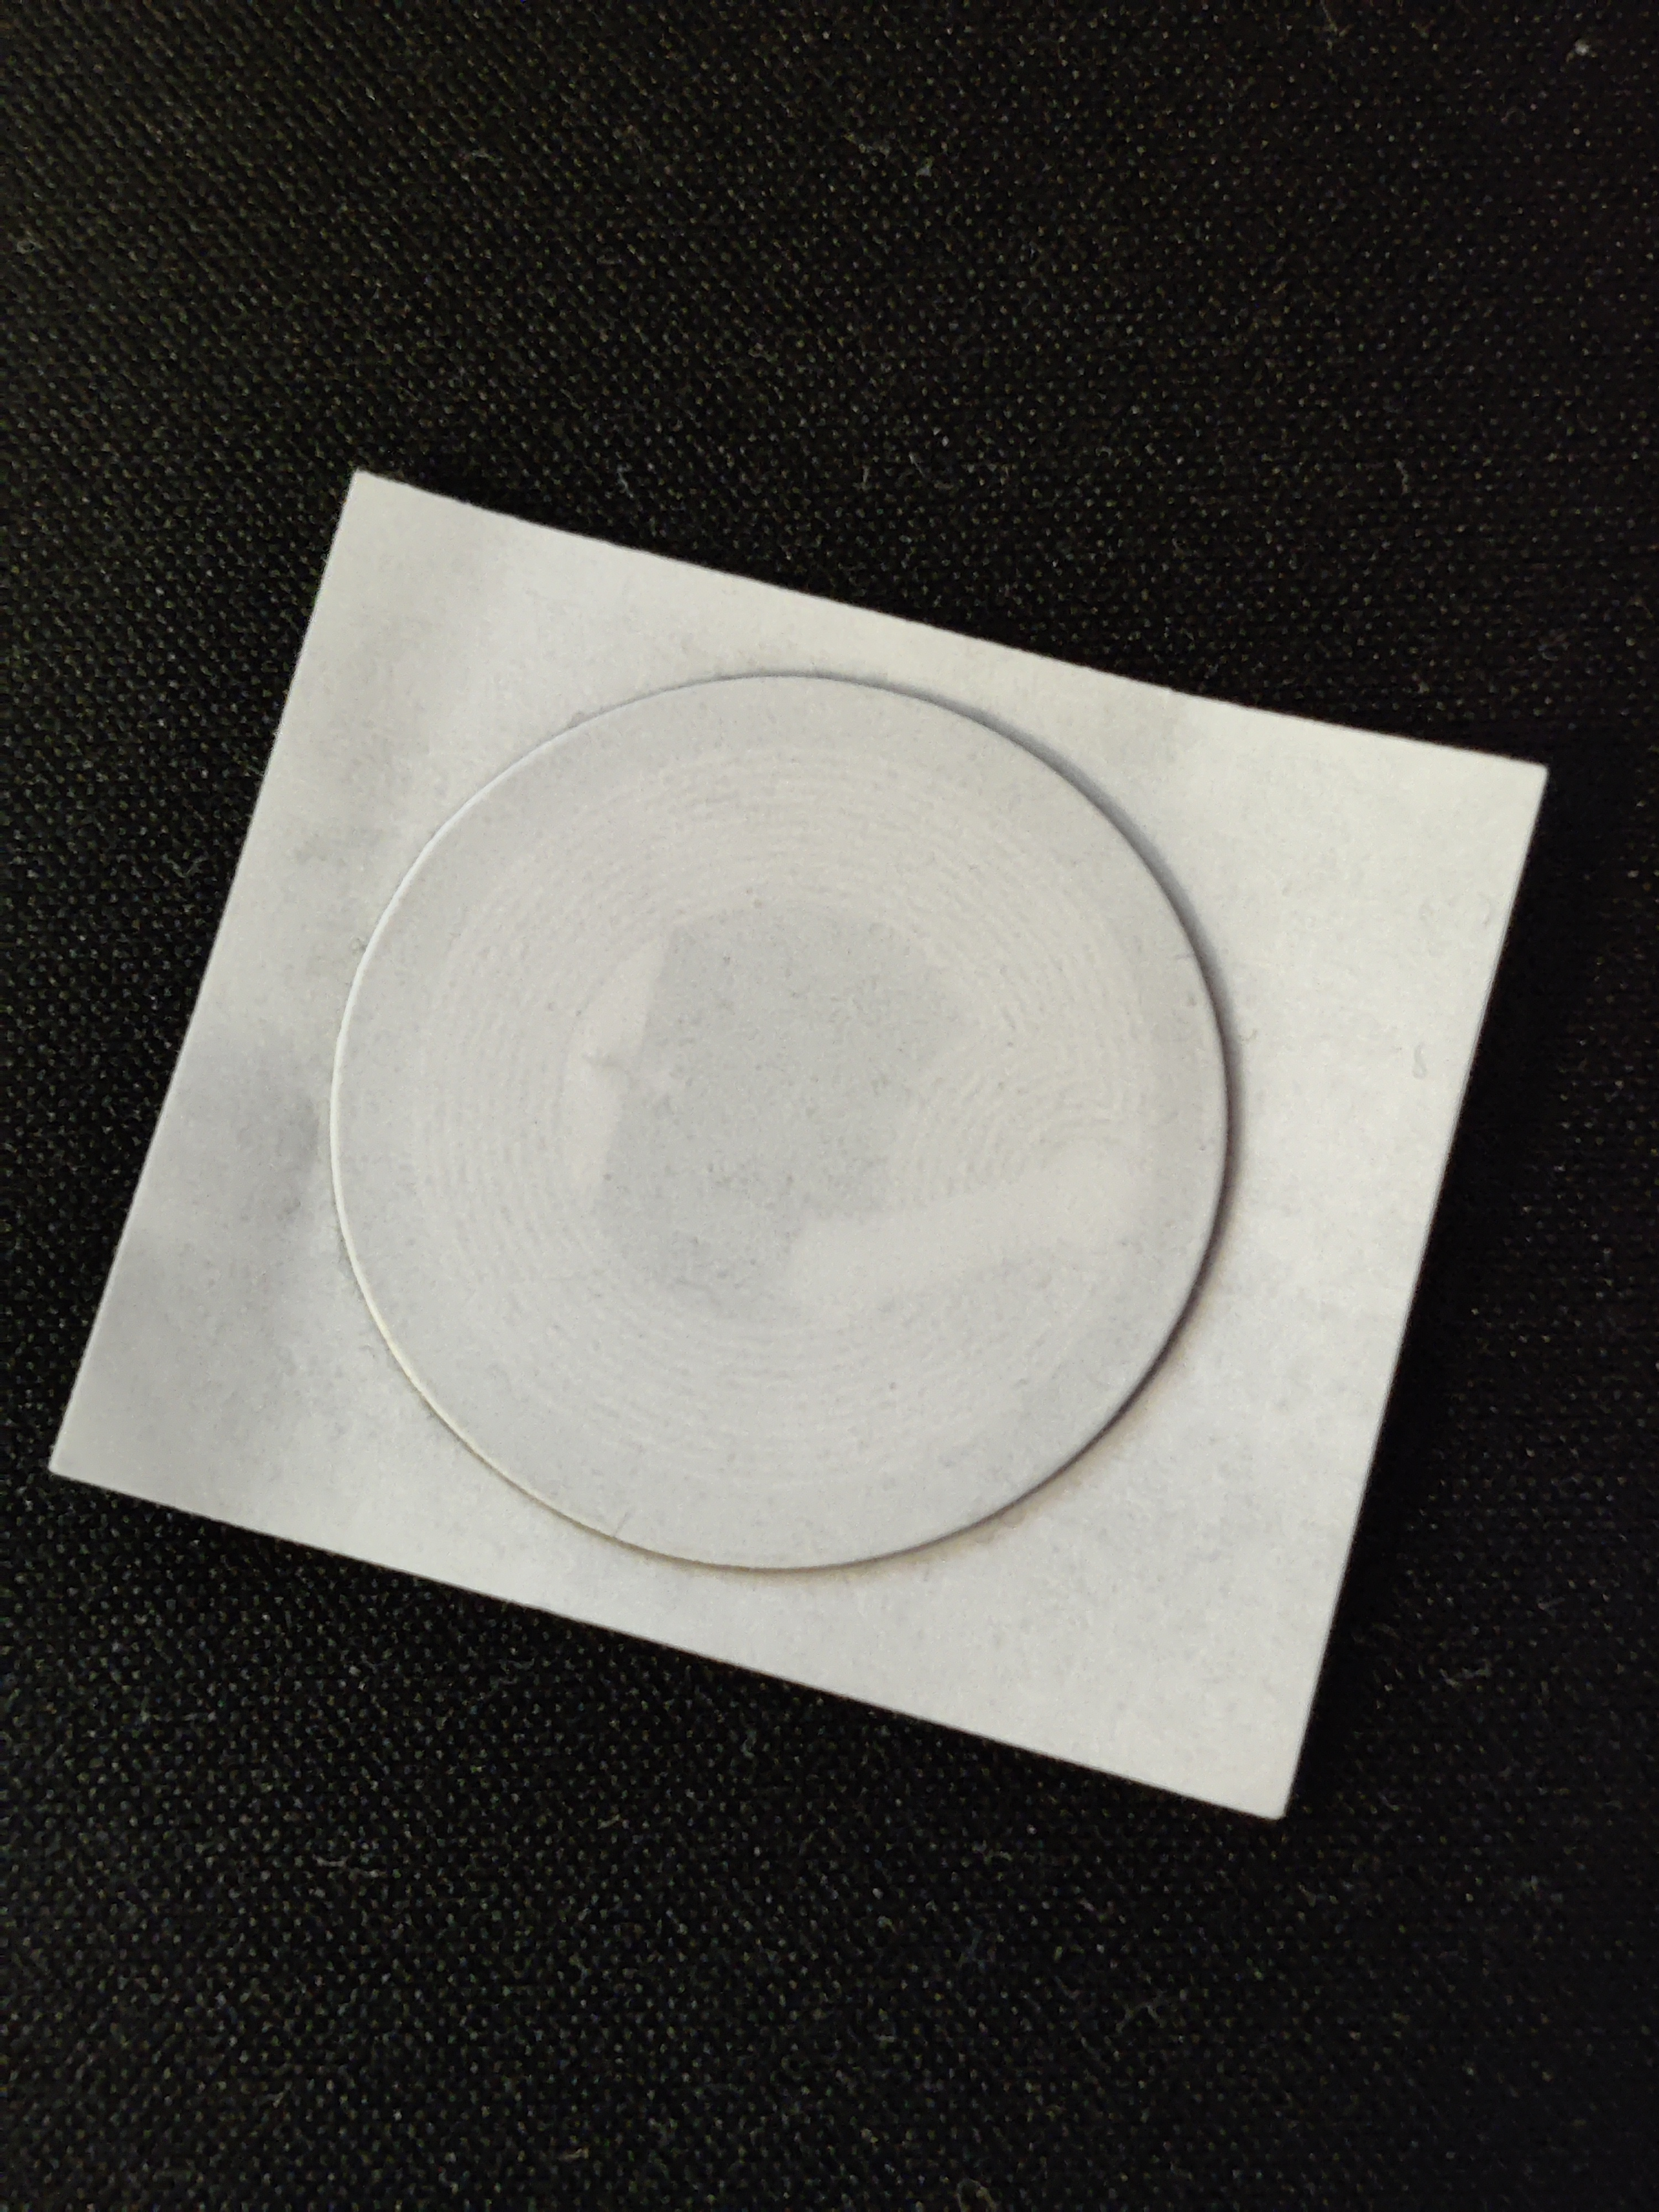
\includegraphics[width=0.4\textwidth]{figures/nfc_tag.jpg}
\caption{NFC Tag}
\label{fig:nfc-tag}
\end{figure}

As a result of a NFC event an exchange of data is being done, for example: in case of a phone communicating with a NFC enabled point of sale (POS, can be seen in figure \ref{fig:pos}) the phone will send the card information needed in order to complete that specific transaction and it will receive a confirmation from the POS. The contactless payments is merely one of the many amazing things that can be done using the NFC technology though.

\begin{figure}
\centering
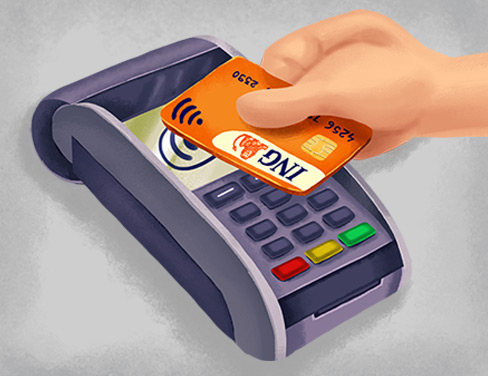
\includegraphics[width=0.4\textwidth]{figures/pos.jpg}
\caption{Point Of Sale (POS) \cite{posImage}}
\label{fig:pos}
\end{figure}

\section{NFC Android}
\label{sec:ch2sec2}

\par The first device to provide NFC functionality was the Nokia 6131 phone in 2006. However the Android operating system was only introduced in 2008 and it took 2 years for an android phone to be equipped with NFC support and the first android phone to do it was Samsung's NEXUS S, released in 2010.

As it is mentioned in \cite{nasution2012prototype}, the function of NFC was introduced by Google into Android 2.3 (API level 9) device. In Android 2.3, the ability of device is limited in only reading the tag. In Android 2.3.3 (API level 10), data writing and trading ability through mode Peer to Peer (P2P) began to be implemented within android devices. 

The uses of the NFC in the Android space are vast and useful in many different ways. One of those is of course the Google Pay system which allows you to make contactless payments with the cards saved into your Google accounts. There was another very interesting feature in Android, called Android Beam which allowed you to transfer files between two NFC enabled Android devices just by touching them one to the other. However, this was deprecated with the introduction of Android API level 29 (also known as Android Q or 10) and replaced with Google's new addition, Nearby Share, which is a direct response and competitor to Apple's AirDrop.

File transfers and contactless payments are merely the top of the iceberg though, the more interesting thing about it comes when you add into the equation the NFC tags. Those can easily be written to with free applications from the Google Play Store, such as TagWriter which allows you to store information or even different commands on the tags. You can use them to store contacts, web pages, or WiFi connectivity information in a manner that when you tap such a tag your device will automatically prompt you to connect to the specific network that has been stored on that specific tag without the need for you to introduce a password (as long as you are in the range to do so, of course).

Another very frequently used functionality of the NFC on Android devices is for pairing bluetooth devices with the mobile phone, such as NFC and bluetooth enabled speakers or even cars. The possibilities are limitless as you can implement custom functionalities.

When NFC was first introduced there were serious concerns about security and privacy, however Google gave the users full control on whether their device can read and receive information throughout the NFC functionality or not by simply adding a toggle button in the quick settings, similar to the WiFi toggle button, see figure \ref{fig:nfcToggle}.

\begin{figure}
\centering
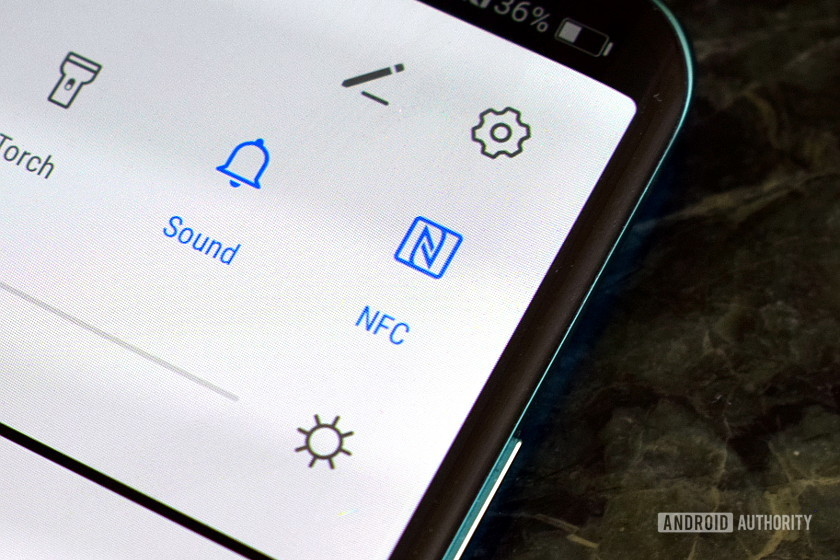
\includegraphics[width=80mm]{figures/nfc_toggle_button.jpg}
\caption{The NFC Toggle button on an Android device \cite{howToUseNfc}}
\label{fig:nfcToggle}
\end{figure}

\section{Usage of NFC in health and other domains}
\label{sec:ch2sec3}

\par As stated in the sections \ref{sec:ch2sec1} and \ref{sec:ch2sec2} one of the domains where the Near Field Communication technology thrives is payments. It was first introduced in the so called contactless cards, which is just a simplified name, easier to recognize by the public, for a Near Field Communication (NFC) enabled card. Those were a serious security concern and people would be skeptical about them as a result of the fact that to make a payment you wouldn't be required any extra information, like the PIN code you would be required to introduce in order to confirm a normal card payment. However this was not true, at least not entirely, as payments without introducing a PIN code in order to confirm the transaction were not allowed past a certain amount, chose by the card issuer.

The NFC technology is also being used in ticketing and loyalty services such as bus tickets that are stored on an NFC enabled card, or loyalty cards that provide you with points that can be spent in different shops. It is also used in special card keys in order to provide you access in some rooms, like in hotels.

According to \cite{lazaro2018survey}, the inductance (and the corresponding capacitance) chosen in the tag design has an important role in the energy harvesting and the loading effects between the tag and reader. This interest in passive NFC sensors led manufacturers of integrated circuits to present several ICs (integrated circuits) with energy harvesting, thus demonstrating the potential market for this technology.

In accordance with \cite{steffen2010near}, if we have a car key with a NFC Interface, where the NFC interface is located inside the car’s key (connected to the key electronics), then one exemplary use case is the Car Status. When a user turns off the car, the car transmits status information to the key via the internal radio interface. When the user is outside the car, he can use a NFC mobile phone to read this information from the key like the status of the locks, the position of the car, the tank level etc.

A new functionality that Apple and Google both announced in the last year is the ability to store your car key on your phone, in order for you to be able to use your phone to unlock and start the car. However, the cars are not NFC enabled by default, so you would need a car that supports this technology in order to take full advantage of it. This will be widely available starting with Android 12, according to Google (figure \ref{fig:google-car-key}).

\begin{figure}
\centering
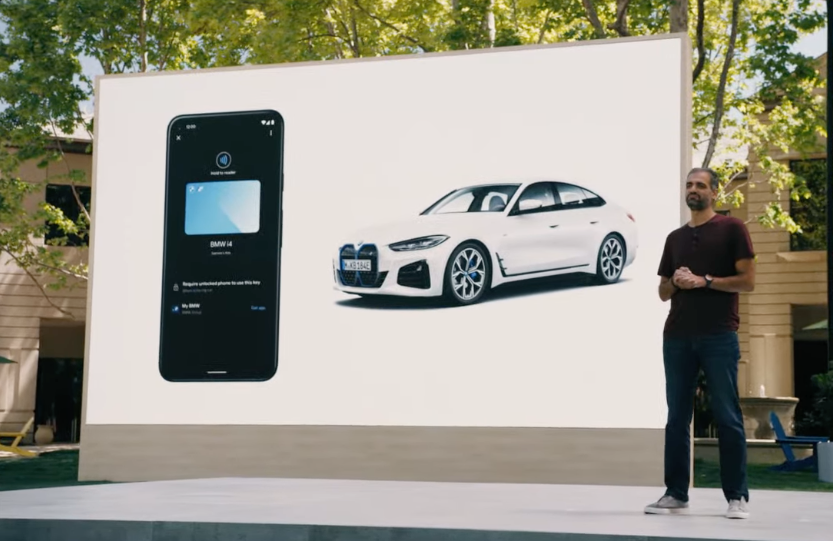
\includegraphics[width=\textwidth]{figures/google_car_key.png}
\caption{Google car key solution \cite{carKey}}
\label{fig:google-car-key}
\end{figure}

Consumers who own car models that have enabled NFC technology, or near-field communication, will be able unlock their car by tapping their phone against the door. The phone communicates with an NFC reader in the user’s car, which is typically located within the door handle. Google said users will also be able to securely and remotely share their car key with friends and family if they need to borrow the car. \cite{carKey}

When it comes to health care the NFC technology is not yet used, however there are studies that explore the ways RFID (Radio-Frequency Identification System) and NFC (which is an RFID based technology) could be used in order to make certain parts of the patient treatment easier and more error-free. One of those parts is actually the medication which is prone to errors due to it being quite demanding in the way it should be administrated. The safe medication care is based on five ”rights”: right medication, right patient, right dosage, right way of taking medication, and right time. \cite{lahtela2008rfid} Using the NFC technology three of these "rights" would be quite easy to accomplish, those being the right patient receiving the intended medication in the prescribed dosage.

Figure \ref{fig:nfc-medication-system} shows how RFID could be used in medication care combined with the electronic patient record and a data system. Tags are placed onto the patient and onto the medication, which information the nurse reads with RFID reader. Next the information is transmitted to the data system for handling, from which the data finally continues to the electronic patient record and to the nurse. The information, which is automatically read from the medication and from the patient to the electronic patient record, improves the surveillance of medication care. \cite{lahtela2008rfid}

\begin{figure}
\centering
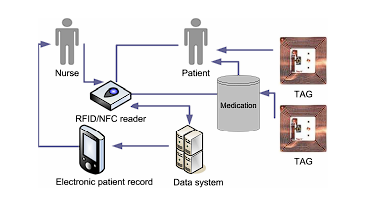
\includegraphics[width=0.75\textwidth]{figures/nfc_medication_system.png}
\caption{Using RFID/NFC in medication care combined with electronic patient record \cite{lahtela2008rfid}}
\label{fig:nfc-medication-system}
\end{figure}

The above scenario is just the start of what we can accomplish in the health care system using the NFC technology and stopping here would be a stupid thing to do. So what else can be done? Well the patient's tag could also contain other information than the prescribed medication alone and with a centralized server this could be just a reference to an entire database of information on one patient alone, including potential allergies, past interventions, blood related information and many other.

\section{Alternative to NFC usage in the Health Tech space}
\label{sec:ch2sec4}

\par As we stated in section \ref{sec:ch2sec3}, the Near Field Communication technology is not really used yet in the Health Tech space, not on a large scale anyway. This started us wondering, if not NFC, what are the alternatives used in this domain? As we were looking for any kind of answers we stumbled across iNTERFACEWARE and some other Electronic Medical Records (EMRs).

iNTERFACEWARE is a company that tries to help the hospitals and the public health agencies in storing their data securely while offering some integration solutions for their Iguana integration engine. Iguana is an amazing engine tool that was build specifically to meet the needs of today's medical system.

Alternatives to Iguana (by iNTERFACEWARE) are considered to be Adverity, EDI HQ and Workato. However none of the above are directly targeted towards the healthcare system. Adverity is targeted towards marketers in order to tackle their data challenges, EDI HQ is mainly designed to support clients in Retail, Logistics and, between others, Healthcare Industries. Workato is a workflow automation system designed for domains like HR, IT, Marketing and others. As a result of the mostly nonexistent alternatives we are either left with iNTERFACEWARE or some EMR solution provided by the Government (if there even exists such a thing).

While having the information stored on a remote server and accessible from certified laptops and desktops on a specific private network inside a medical center may be secure, getting those medical records and reports to the nurses or some other medical personnel is still a tedious job to accomplish using printed reports that are in some cases left at the bed of the patient or have to be requested every time from an information center in the hospital.

We can safely state that, even though EMR are a great solution for storing the information about patients in a secure way, the usage of printed reports that can sometimes be viewed or accessed by some random unauthorized person kind-of defeats the purpose of EMRs in the first place. We are not saying that those systems are not good, or not an appropriate solution, however we are saying that they are not enough by themselves and that those systems do not solve the entire problem on their own.

\section{Privacy concerns}
\label{sec:ch2sec5}

\subsection{Privacy in general}
\label{sec:ch2sec5subsec1}

\par First of all we need to answer a simple but rather complicated question: what is privacy? In order to answer this we turned over to \cite{solove2008understanding} for a better definition: "Privacy, however, is a concept in disarray. Nobody can articulate what it means. Currently, privacy is a sweeping concept, encompassing (among other things) freedom of thought, control over one’s body, solitude in one’s home, control over personal information, freedom from surveillance, protection of one’s reputation, and protection from searches and interrogations."

In a time where technology thrives and expands at a rapidly increasing rate, data becomes more and more important. As a consequence privacy is harder to preserve with each day passing by. Companies and institutes fight over how much information they can store about us for different reasons - some might be for a quality of service improvement, some for advertisements and other for the exact purpose of selling them and making a profit off of us. We believe that we can think of at least a handful of companies that do this. Let's take for example the three giants of the tech world: Google, Apple and Facebook. 

Facebook is by far the worst in the opinion of most people, especially since the Facebook-Cambridge Analytica data scandal from 2018. This specific event triggered a big concern around the world about consumer privacy and the data collected from the users which lead to an improvement in the legal system, especially in the EU, when the General Data Protection Regulation was enacted.

In 2018, the European Union, put into effect its new data protection law. The General Data Protection Regulation (GDPR) is the toughest privacy and security law in the world. Though it was drafted and passed by the European Union (EU), it imposes obligations onto organizations anywhere, so long as they target or collect data related to people in the EU. The regulation was put into effect on May 25, 2018. The GDPR will levy harsh fines against those who violate its privacy and security standards, with penalties reaching into the tens of millions of euros. \cite{whatIsGDPR}

Since this law was enacted there was a serious change in perspective around the world. People were more aware than ever about the importance of their privacy and they started demanding their rights. As stated in \cite{voigt2017eu}, the EU aims at regaining the people’s trust in the responsible treatment of their personal data in order to boost digital economy across the EU-internal market with the GDPR.

As a result of this fact the big giants, Google and Apple, took special steps in order to help preserving users privacy on the internet, but the one that surely affects us all is Google, as its advertisement system is the most used one on the internet. Recently they started working on a new data collection process in order to give users more privacy, while not completely giving up on targeted ads and their relevance to the user.

Google's proposed solution is called the Federated Learning of Cohorts (FLoC) which is supposed to take the place of the cookies we all know and love that you always have to allow in your browser whenever you access a website in order to have the intended experience. FLoC proposes a new way of targeting ads by no longer allowing the business to create a special profile on that person, instead it places a person in a cohort of users with the same interests. In this way you will still get advertisements for things that are relevant to you, but not as personal as before, for example:
if you've searched for let's say a Tesla Model 3 and a BMW i8, which are both electric cars, the algorithm will place you in a cohort of users that are interested in electric cars. As a result the ads targeted to your cohort will contain electric cars, but not necessarily the models you searched for or the brands you've searched for. Still relevant ads, but not as creepy as before.

\subsection{Privacy in the Health Care system}
\label{sec:ch2sec5subsec2}

\par Healthcare organizations store, maintain and transmit huge amounts of data to support the delivery of efficient and proper care. Nevertheless, securing these data has been a daunting requirement for decades. Complicating matters, the healthcare industry continues to be one of the most susceptible to publicly disclosed data breaches. In fact, attackers can use data mining methods and procedures to find out sensitive data and release it to public and thus data breach happens. While implementing security measures remains a complex process, the stakes are continually raised as the ways to defeat security controls become more sophisticated. \cite{abouelmehdi2017big}

We can see that we as a society started evolve in this specific subject of privacy in the last 3 years, yet there are still domains that need to catch up, in a big way. According to GDPR, hospitals have an even bigger than before responsability of keeping our data private from prying eyes and this is not an easy job. In a space where they need to have quick access to our information, the medication that was prescribed to us and other records that are essential for them in helping you get healthy once again, it might be close to impossible to preserve a patient's privacy. 

As noted in \cite{hathaliya2020exhaustive}, nowadays, security and privacy are the primary concern of the healthcare industry because of a tremendous amount of health data accessed and transmitted over the Internet. The internet is basically open to everyone in order to communicate and search for information, so as a result there is a possibility of various attacks on the data. In order to respond, the specialists started using cryptography as a counter-measure to those attacks.

Privacy of information collected during health care processes is necessary because of significant economic, psychologic and social harm that can come to individuals when personal health information is disclosed. \cite{barrows1996privacy} This is not an easy challenge and establishing such an implementation of security policies can be quite demanding in an Electronic Medical Record (EMR) system. However one of the goals we are trying to achieve with EMRs is to ensure the availability of health data for authorized persons and the prevention of unauthorized or unintended withholding of information or resources \cite{barrows1996privacy} which in our opinion is worth fighting for.

Until now, whenever someone was hospitalized they would keep some medical reports around your bed, which contain different information about the patient, like her/his current condition, some personal information and the treatment or medication they are supposed to receive. The medical reports were around their bed to make it easier for the nurse and the different doctors to communicate about how the patient's situation is evolving. Today that is not a solution anymore, privacy is important and, not respecting it, punishable in Europe. Also a file about a patient near their bed can easily be accessed by someone unauthorized or ill intended, which represents a security threat to the data collected by that specific health institute.

As we stated in section \ref{sec:ch2sec4} there are no complete solutions to this issue at this point. We took a look throughout a catalog of mobile applications that could even come close to a potential solution to this problem an we could only find some medical records applications for mobile devices, like the Multi-Profile Medical Records application found on the Google Play Store, but those were never built nor intended to be used by a medical institute. Those applications were intended to be used by the patient to take notes for themselves, so once again those do not present a solution for the exact purpose of our problem.

\subsection{Privacy concerns when using NFC in Health Tech}
\label{sec:ch2sec5subsec3}

\par One of the main concerns when using the NFC technology when it comes to privacy is the fact that the NFC tags can be read by any device with NFC reader capabilities. There is no way to make the information private in a way that only authorized devices could read those tags. While this is indeed true and it is a real problem it can be easily mitigated by encrypting the data stored on this tags or by not storing any sensitive data on them, in a way that only a person with authorized access to the server can access the private information.

Let us suppose though that an authorized device reaches the hands of an unauthorized person which can lead to leaks of information and that person having access to the database through the mobile application. In order to solve this issue a possible solution could be a Two Factor Authentication (2FA) system, where after a successful tag read an extra step would be required in order to access the information, for example the device's PIN code, pattern, fingerprint or face recognition, depending on the user's device settings.

Another privacy/security concern is what if one person from the medical personnel, so someone with authorized access, decides to leak some information by screen-recording or taking screenshots of patient's information or of some medical reports? Is there a way to mitigate such actions? The answer to those questions is yes, there is a solution. The Android operating system provides us with a flag (FLAG\_SECURE) that can be used in order to make those actions impossible. 

How does it work? The operating system will completely deny your possibility of taking screenshots on screens that have this flag attached, while in the case of screen recordings you would be able to actually perform this action, whenever you enter those flagged screens the screen recording will have a black overlay over the content from those screens so no information would be leaked. 

What about the preview that the system shows us when we open the recent applications screen? This, as well, is considered secured. As a consequence whenever you put the application in background and open the most recent applications, if the last opened screen was a secure flagged screen you would not be able to see any preview of the screen's contents, instead you would be presented with a white screen as a preview.

\section{Proposed solution}
\label{sec:ch2sec6}

\par We thought about what was the best approach to our issue, taking into account the fact that it has to be easy to implement and handy to use in order to make the integration as simple as possible and with the smallest cost possible while also being easy to use by any authorized medical personnel. We came up with a really interesting solution which takes advantage of the fact that most Android powered phones have NFC capabilities these days.

In our solution we did not focus on the server side of the issue, as there probably is already some EMR integration in a medical institute. Instead we focused on the mobile application to provide an idea of what could be possible with some basic Application Programming Interface (API) end-points that are pretty easy to implement on the server side.

The solution that we are proposing takes advantage of the already implemented bracelets in hospitals, by including an NFC Tag in those bracelets. Those tags will contain a database ID, with no meaning to any person that doesn't have access to the database or real life reference to that person.

The medical personnel would be allowed to see old reports and generate new ones for a specific patient, nurses would be able to register a new patient and write the id to the bracelet's tag. There is a lot of space for developing new use-cases and help the users have specialized options based on their assigned role in the application. We believe that this solution would help the medical professionals have an easier time being up to date with every single report that's being generated when visiting the patient, thus making their work a tad bit easier.
\chapter{Architectures and Frameworks}
\label{chap:ch3}

\section{Mobile application}
\label{sec:ch3sec1}

\par We have decided to write the entire mobile application in Kotlin and use the Model-View-ViewModel (MVVM) architecture in a combination with Koin as our dependency injection tool. To accomplish the reading of data from the bracelets we will use the default NfcAdapter provided by Android as it is a reliable way to achieve our goal of retrieving the information from those tags.

MVVM is our go for the mobile application architecture because it is currently considered to be the best choice in the case of Android applications since it is easy to adapt in most scenarios. This architecture helps us write more reusable code (if used right) and gives us flexibility in changing our user interface without necessarily having to refactor other logic in the code base.

A good and comprehensive definition of the MVVM theory can be found in \cite{anderson2012model}, and it states: "At the heart of the MVVM design pattern is the separation of a view’s logic from its look. Instead of having a mass of code in a View’s code-behind, much of this code will be extracted out into a ViewModel class separated from the View itself. This ViewModel class will then expose data and operations publicly for one or more Views to consume. The result of this will be that the view should have very little code-behind. You can then use data bindings and commands/behaviors as the glue to connect the View and the ViewModel together."

The architecture consists of three layers: Model, View and ViewModel, which we are going to tackle separately and it can be seen in figure \ref{fig:mvvm}. An example of how the architecture is used in our project can be seen in figure \ref{fig:mvvm-project-example}.

\begin{figure}
\centering
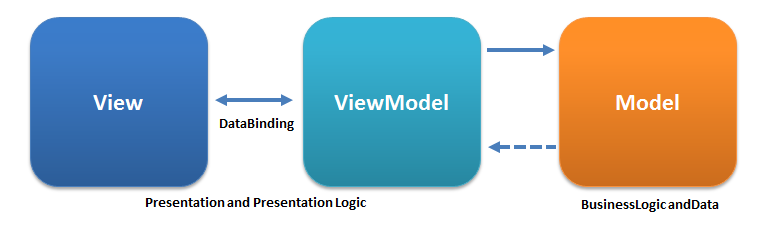
\includegraphics[width=\textwidth]{figures/fig_3_1.png}
\caption{The MVVM architecture \cite{mvvmPattern}}
\label{fig:mvvm}
\end{figure}

\begin{figure}
\centering
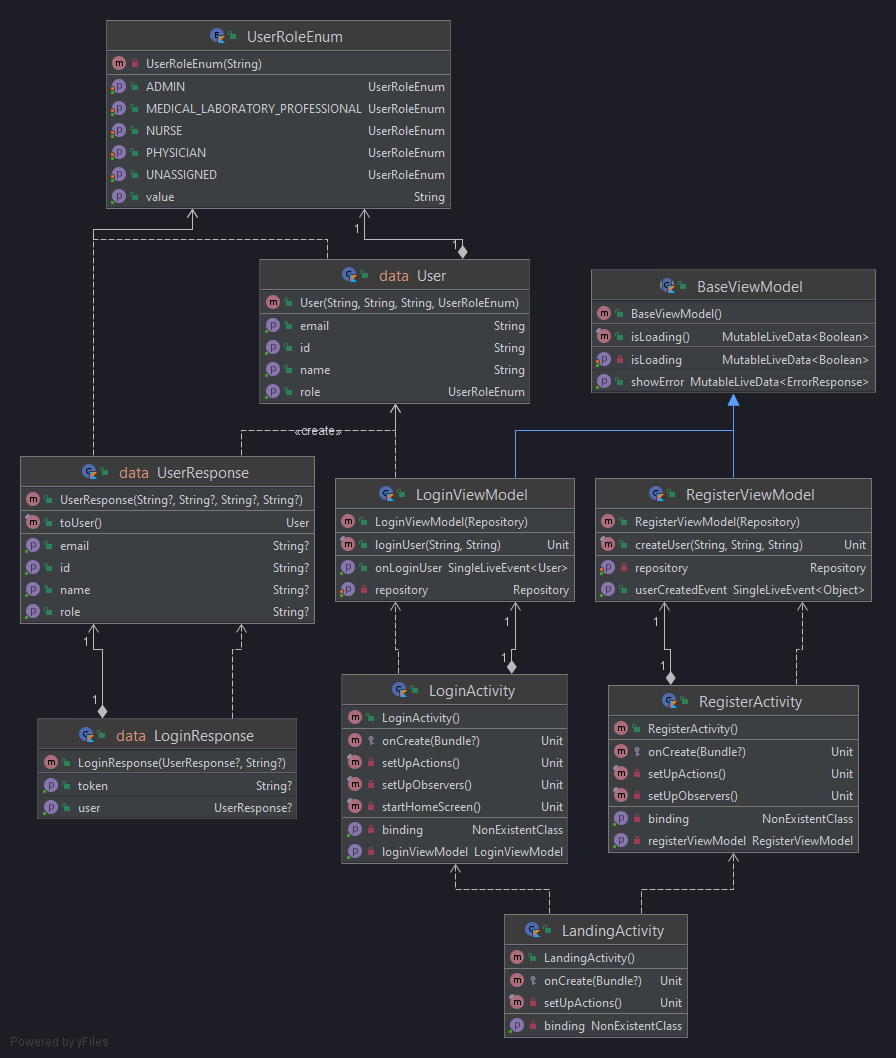
\includegraphics[width=\textwidth]{figures/mvvm_project_example.png}
\caption{The UML class diagram for the Sign Up and Sign In use-cases to exemplify the MVVM architecture of the project}
\label{fig:mvvm-project-example}
\end{figure}

\subsection{The Model}
\label{subsec:ch3sec1subsec1}

\par Let us begin with the basic building block which is a key component for all applications, concretely: information and data. Those are stored in the model. The model is basically the domain object and it represents the actual data and/or information that is used throughout the application. A basic example of such a model could be a user, which would contain an ID, a name, an email address and an assigned role, as seen in figure \ref{fig:user-uml}.

\begin{figure}
\centering
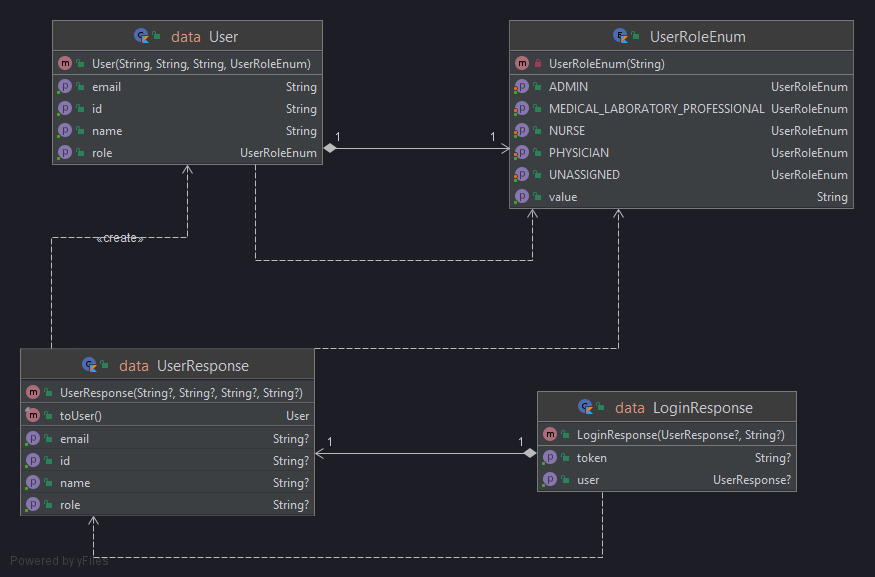
\includegraphics[width=\textwidth]{figures/user_uml.png}
\caption{The UML class diagram for the User model}
\label{fig:user-uml}
\end{figure}

The most important thing about the model that we should keep in mind is that it holds the actual data and information, but not the logic or services that process it. The model should not be responsible for fetching data from a server or formatting text to display on the screen. However there are some exceptions where some models do contain some business logic like validations, but typically this should be separated from the model.

\subsection{The View}
\label{subsec:ch3sec1subsec2}

\par The view is basically the only interactable part of our application to the end user, the user interface, or the way we present our data. The view manipulates the data and formats it in order to make it easier to be consumed by the end user. As a quick example we have a date that might be stored as a timestamp that looks something like "2021-05-31T01:48:52Z" in our model, while for the end user it will be displayed as the year, month, day, hour, minute and second in their specific timezone. Also, a view can have associated behaviors with it, like for example accepting some user input through input text fields for your email and password. It manages inputs which in the end change properties in the model.

As opposed to some other architectures, the view in MVVM is active, which means that it doesn't completely turn over the control of its state to the viewmodel / controller / presenter. The view is responsible of its own events, contains behaviors and data-bindings which in the end needs to know about the underlying structure (the model and the viewmodel). Sure the events might be mapped to some commands or method calls, but the view is still responsible, in the MVVM architecture, of handling the events that belong to it.

However, an important note is that the view is still not responsible of maintaining its state, it should synchronize it with the viewmodel, about which we will talk next.

\subsection{The ViewModel}
\label{subsec:ch3sec1subsec3}

\par The viewmodel is our controller, or presenter if you want. It is the key piece of the architecture that helps keeping the view separated form the model. In this way the model does not need to be aware of the users view of the data, and instead it only holds the information, while the view holds the formatted information. The viewmodel behaves like a link between them.

The viewmodel will maybe interact with a service in order to retrieve the model in order to format the information and pass it to the view, or it might take an input from the view in order to pass it to the model. It also exposes methods, commands, and other points that help maintain the state of the view, manipulate the model as the result of actions on the view, and trigger events in the view itself. \cite{viewmodel}

\section{Server application}
\label{subsec:ch3sec2}

\par To write our server applications we have decided to use the new Kotlin for servers plugin created by JetBrains called Ktor. As for the database we have chosen PostgreSQL as there are easy integrations between it and Ktor made possible by some frameworks provided by JetBrains.

\subsection{Ktor}
\label{subsec:ch3sec2subsec1}

\par Ktor is an asynchronous framework for creating microservices, web applications, and more. It’s fun, free, and open source. \cite{ktor}

First of all we have chosen to use Ktor because of our familiarity with Kotlin, coming from a mobile development background. However, that was not the only reason. Ktor provides us with a very simple way of creating a server by taking the responsability of running asynchronous tasks in its own hands.

The syntax in Ktor is very simple and simple to understand. It uses some install statements in order to build some components by default, taking a lot of work off of our shoulders and removing a lot of so called boiler-plate code from the project, some examples would be the default headers that should be attached to every response, the error handling and the JSON content negotiation. The code for all of those can be seen in figure \ref{fig:install-statements}.

\begin{figure}
\centering
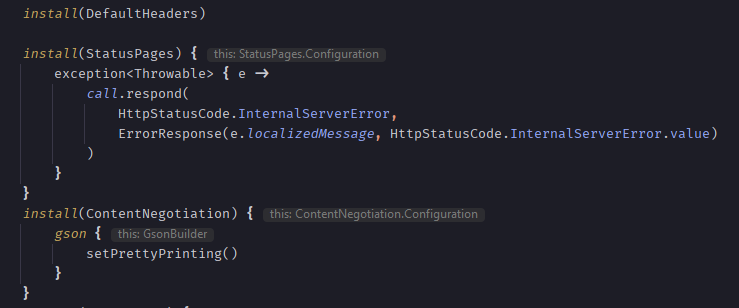
\includegraphics[width=\textwidth]{figures/install_statements_snippet.png}
\caption{Ktor install statements code snippet}
\label{fig:install-statements}
\end{figure}

\subsection{PostgreSQL}
\label{subsec:ch3sec2subsec2}

\par The reason for which we have chosen PostgreSQL is because it is very easy to be integrated with Ktor by only using three (3) main frameworks. Those frameworks are the following: the Exposed Object-relational mapping (ORM) library, the Java Database Connectivity (JDBC) Connection Pool HikariCP library and the Java Database Connectivity (JDBC) Connector for PostgreSQL.

The Exposed library is used in order to map the database tables into Ktor readable objects that can be interrogated easily with a Kotlin-like syntax. Take for example the getUserById method from figure \ref{fig:getUserById}, where Users represents a so called UUID (Universally Unique Identifier) Table, a table for which the IDs are auto-generated as UUIDs (figure \ref{fig:users-table}).

\begin{figure}
\centering
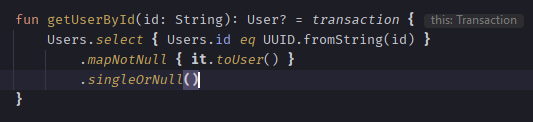
\includegraphics[width=0.75\textwidth]{figures/get_user_by_id.png}
\caption{Exposed syntax example for interrogating the database}
\label{fig:getUserById}
\end{figure}

\begin{figure}
\centering
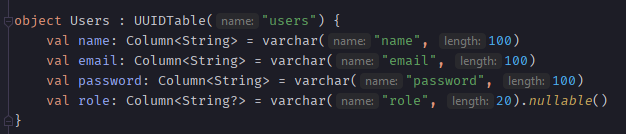
\includegraphics[width=0.75\textwidth]{figures/users_table_example.png}
\caption{Exposed syntax example for the Users table definition}
\label{fig:users-table}
\end{figure}

The Hikari Connection Pool library provides us with an easy way to configure the connection to the actual database. It only requires a configuration file which we pass to its constructor and we are good to go.

The PostgreSQL library is only included for support in order to connect to the database using Hikari.
\chapter{Application requirements}
\label{chap:ch4}

\section{Android application requirements}
\label{sec:ch4sec1}

\par For our application the minimum SDK version is 23. This means that any Android device that has an Android version greater or equal to 6 (code named "Marshmallow") will be able to run our application. However there is a second requirement and that is to have NFC capabilities.

\section{Server application requirements}
\label{sec:ch4sec2}

\par Our server runs on Ktor, but there are no specified system requirements for it. However it requires an IntelliJ IDEA Ultimate as it is a proprietary plugin for Kotlin made by JetBrains. The requirements for the IDE are shown in figure \ref{fig:requirements-intelij}.

\begin{figure}
\centering
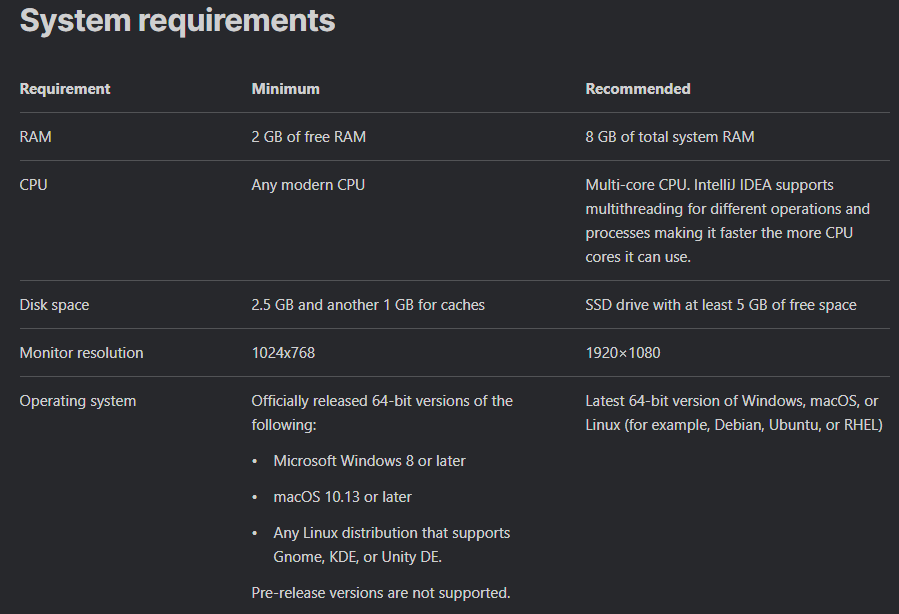
\includegraphics[width=\textwidth]{figures/system_requirements_intellij.png}
\caption{The system requirements for IntelliJ IDEA. \cite{intellijIdea}}
\label{fig:requirements-intelij}
\end{figure}

The server application also uses PostgreSQL 13.2 for its database. The requirements for this version were not made public, however we were able to find the system requirements for the previous version (12.0) so we will suppose that those stayed the same. The requirements can be seen in figure \ref{fig:requirements-postgresql}.

\begin{figure}
\centering
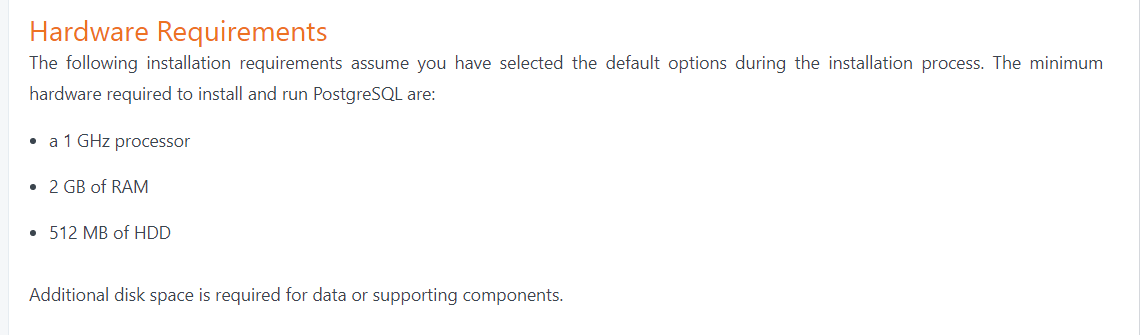
\includegraphics[width=\textwidth]{figures/postgresql_requirements.png}
\caption{The system requirements for PostgreSQL 12.0. \cite{postgresSql}}
\label{fig:requirements-postgresql}
\end{figure}
\chapter{User Manual}
\label{chap:ch5}

\section{Account setup and role assignment}
\label{sec:ch5sec1}

\par When first opening the application the user is taken to a Landing screen (as seen in figure \ref{fig:landing-screen}) where he or she would be presented with the option to Sign Up for a new account or Sign In in an existing account. When pressing the Sign Up button is pressed the user is taken to the Sign Up screen where he or she can send a registration request for a new account, as seen in figure \ref{fig:sign-up-screen}.

\begin{figure}
\centering
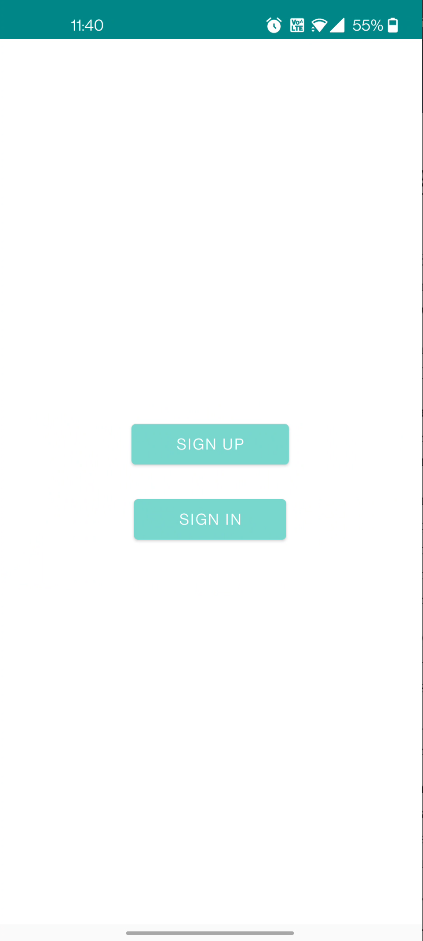
\includegraphics[width=0.4\textwidth]{figures/landing_screen.png}
\caption{The Landing screen}
\label{fig:landing-screen}
\end{figure}

\begin{figure}
\centering
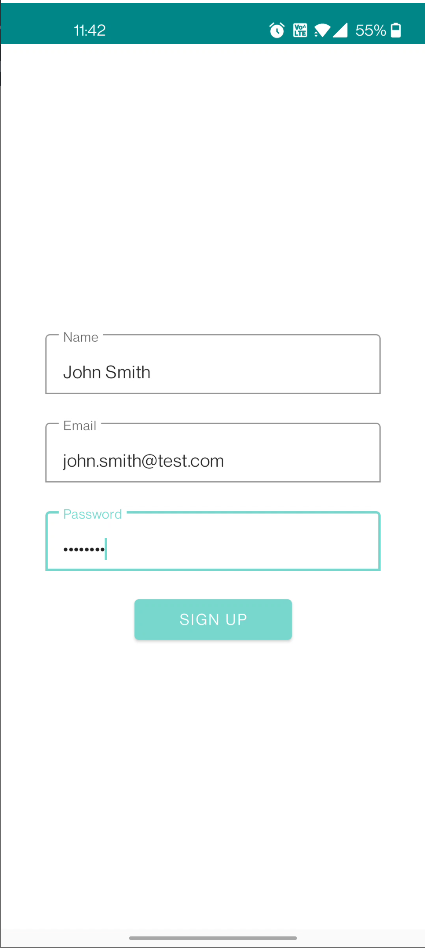
\includegraphics[width=0.4\textwidth]{figures/sign_up_screen.png}
\caption{The Sign Up screen}
\label{fig:sign-up-screen}
\end{figure}

Once this registration is completed, however, the users are still not yet allowed to login into the application as their account needs to be assigned to a specific role. The available roles are the ones seen in the figure \ref{fig:user-role-enum}, except the admin role which is a special role only used to access the dashboard. The admin is the only role that gives an user access to the dashboard where roles can be assigned. The role selection process for our newly created user can be seen in figure \ref{fig:dashboard-assign-role}.

\begin{figure}
\centering
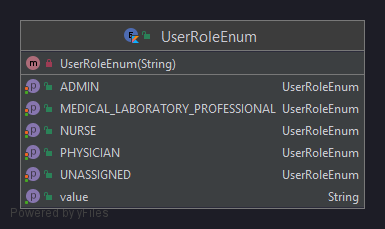
\includegraphics[width=0.75\textwidth]{figures/user-role-enum.png}
\caption{UserRoleEnum Class Diagram}
\label{fig:user-role-enum}
\end{figure}

\begin{figure}
\centering
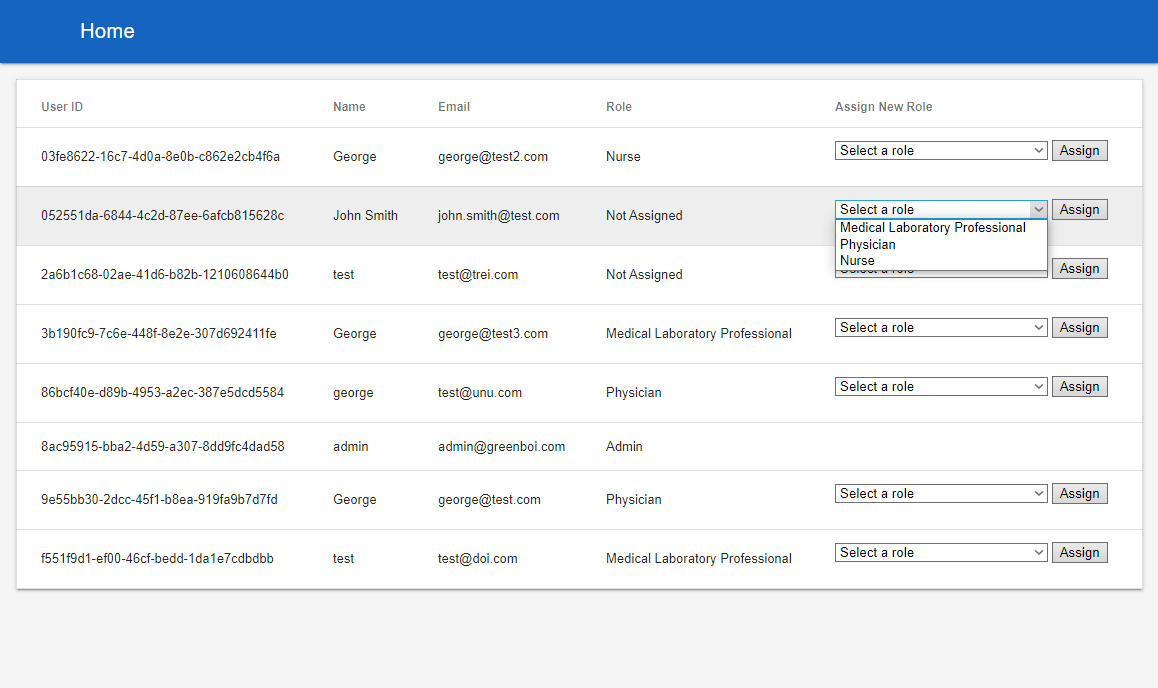
\includegraphics[width=\textwidth]{figures/dashboard_assign_role.png}
\caption{The Admin Dashboard}
\label{fig:dashboard-assign-role}
\end{figure}

\section{Sign In and Home Page}
\label{sec:ch5sec2}

\par In order to Sign In the user needs to go back to the landing screen (figure \ref{fig:landing-screen}) and tap the Sign In button. The user now is being taken to the Sign In screen (figure \ref{fig:sign-in-screen}) where he or she is being asked for the login credentials they have previously created. Once inserted, if they tap the Sign In button a request will be made to the server in order to retrieve an authentication token and the current user's profile.

\begin{figure}
\centering
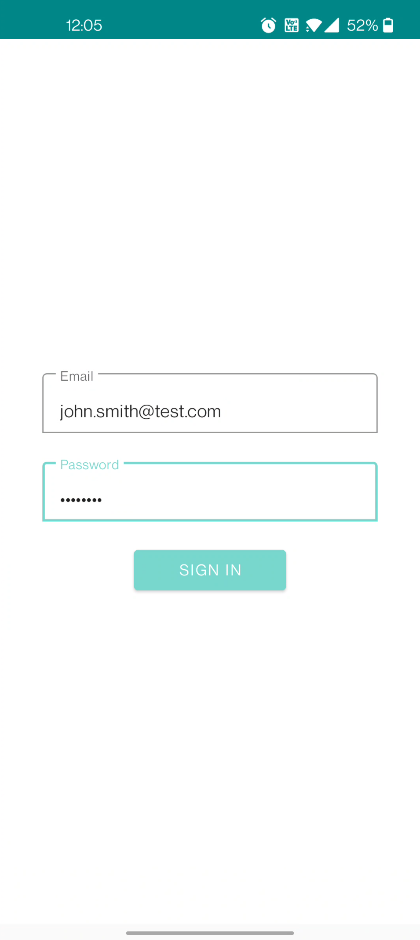
\includegraphics[width=0.4\textwidth]{figures/sign_in_screen.png}
\caption{The Sign In screen}
\label{fig:sign-in-screen}
\end{figure}

After the Sign In process is completed and the required objects are retrieved the user is taken to the home screen (figure \ref{fig:home-screen}). Here the users are presented with some options. The first option is to Sign Out from their account, which, when pressed, will invalidate the user's session and take them back to the landing page. The Second option is to register a patient, which is only available for an account with the Nurse role assigned. The third option is to read a patient's tag.

\begin{figure}
\centering
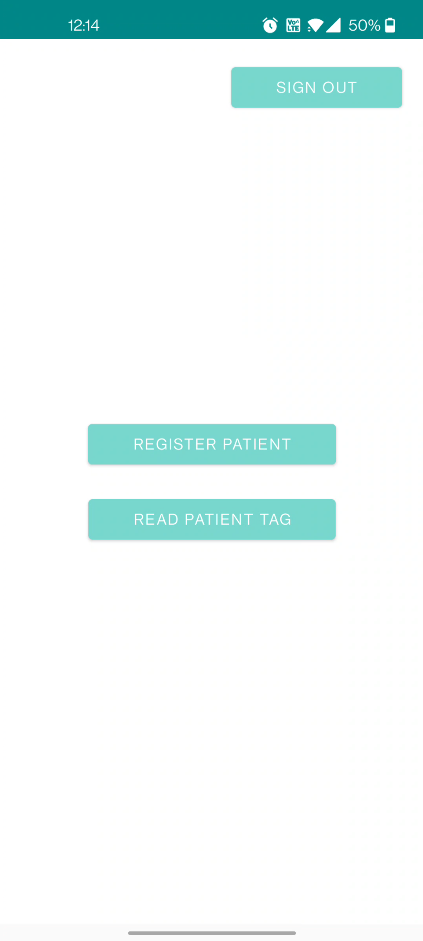
\includegraphics[width=0.4\textwidth]{figures/home_page_screen.png}
\caption{The Home screen}
\label{fig:home-screen}
\end{figure}

\section{Registering a patient}
\label{sec:ch5sec3}

\par When selecting the Register Patient option from the home screen (figure \ref{fig:home-screen}) the user is presented with a form that needs to be completed in order to register a new patient in the database (figure \ref{fig:register-patient-screen}).

\begin{figure}
\centering
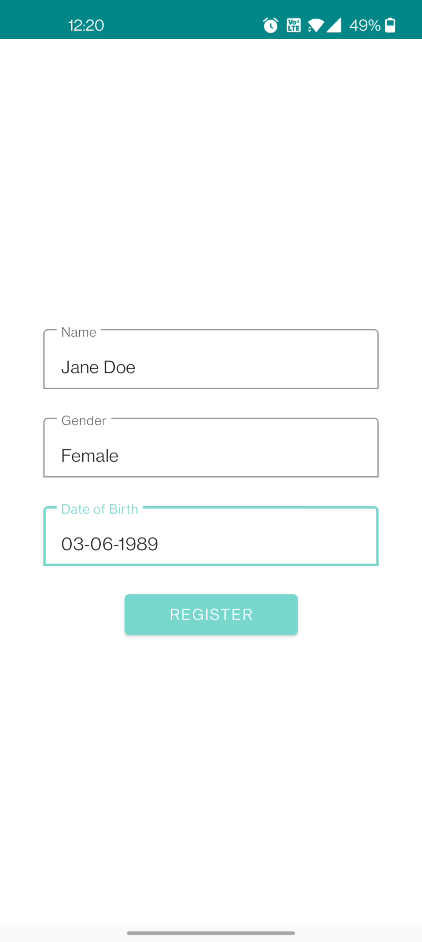
\includegraphics[width=0.4\textwidth]{figures/register_patient_screen.png}
\caption{The Register Patient screen}
\label{fig:register-patient-screen}
\end{figure}

After tapping the register button the nurse is taken to a new screen where she is presented with the possibility of assigning an NFC enabled bracelet to the newly registered patient (figure \ref{fig:write-tag-screen}). As a result of following the instructions that are on the screen the user will be presented with a confirmation dialog, as seen in figure \ref{fig:write-tag-confirmation}. When tapping the Done button the nurse will be automatically taken back to the home page (figure \ref{fig:home-screen}).

\begin{figure}
\centering
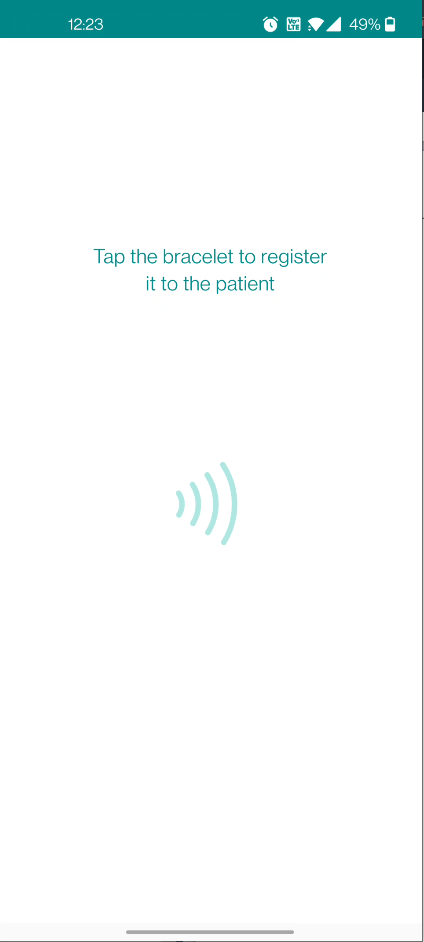
\includegraphics[width=0.4\textwidth]{figures/write_tag_screen.png}
\caption{The Register Tag screen}
\label{fig:write-tag-screen}
\end{figure}

\begin{figure}
\centering
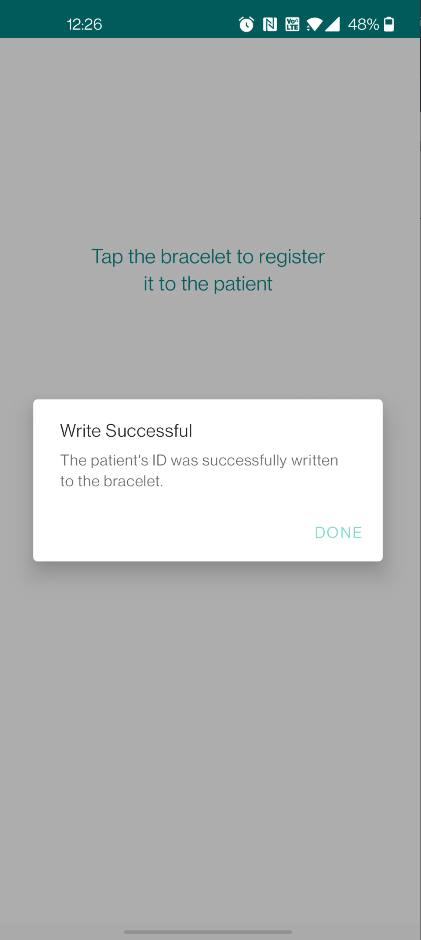
\includegraphics[width=0.4\textwidth]{figures/write_tag_confirmation.png}
\caption{The Register Tag Confirmation}
\label{fig:write-tag-confirmation}
\end{figure}

\section{Retrieving a patient's information}
\label{sec:ch5sec4}

\par In order to retrieve the patient's information the medical personnel is required to tap the Read Patient Tag button found on the home page (figure \ref{fig:home-screen}). Upon doing so, the user is taken to a new screen where he or she is required to close the distance between the device and the bracelet in order to read-off the information from it, as seen in figure \ref{fig:read-tag-screen}. Upon successfully reading the ID stored on the NFC enabled bracelet the patient's information is requested from the server along with a list of generated reports. Once retrieved the user is taken to the View Patient screen (figure \ref{fig:view-patient-screen}).

\begin{figure}
\centering
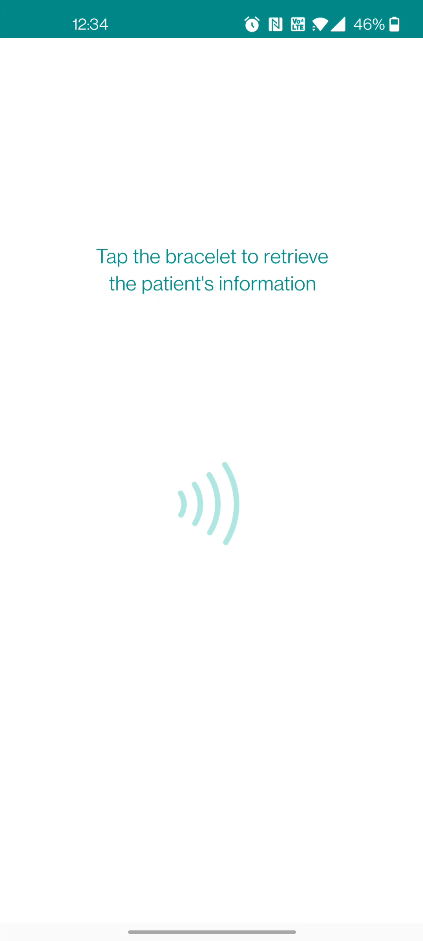
\includegraphics[width=0.4\textwidth]{figures/read_tag_screen.png}
\caption{The Read Patient Tag Screen}
\label{fig:read-tag-screen}
\end{figure}

\begin{figure}
\centering
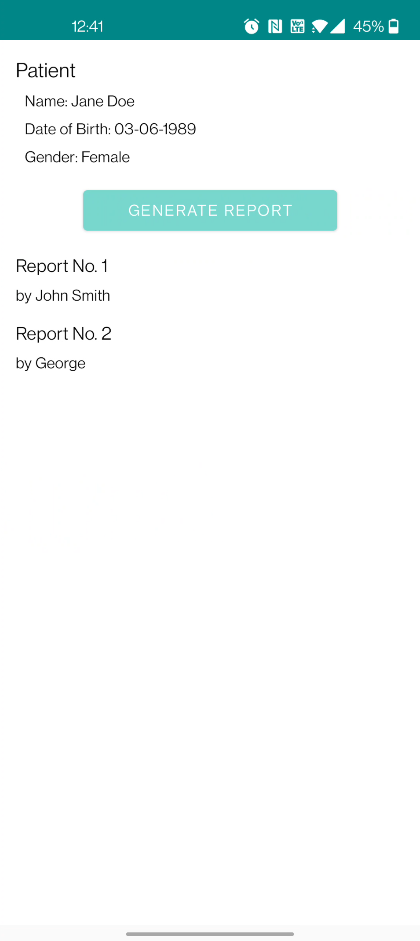
\includegraphics[width=0.4\textwidth]{figures/view_patient_screen.png}
\caption{The View Patient Screen}
\label{fig:view-patient-screen}
\end{figure}

\section{Generating and viewing generated reports}
\label{sec:ch5sec5}

\par When the user is on the View Patient screen, he or she will be able to either view an already generated report from the list seen in figure \ref{fig:view-patient-screen} or generate a new report. Upon selecting a generated report, the details about it are requested from the server and once retrieved, displayed for the medical personnel on a new screen (figure \ref{fig:view-report-screen}).

\begin{figure}
\centering
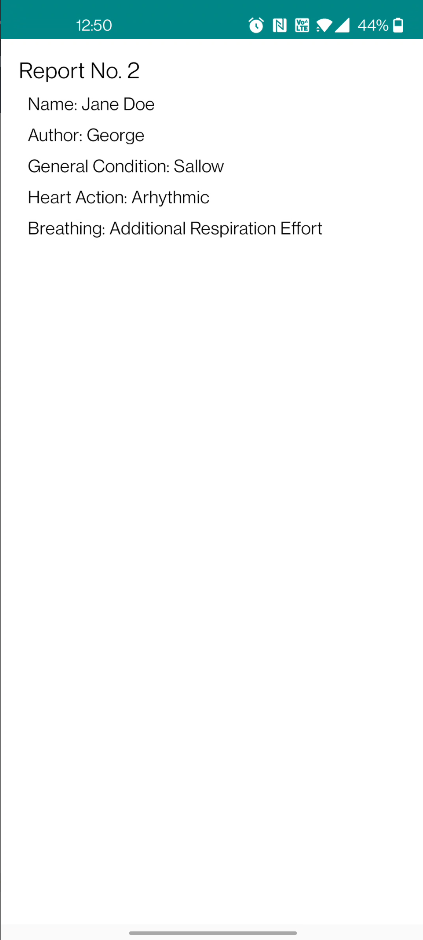
\includegraphics[width=0.4\textwidth]{figures/view_report_screen.png}
\caption{The View Report Screen}
\label{fig:view-report-screen}
\end{figure}

If the medical personnel selects the Generate Report button from the View Patient screen, the user will be presented with a new screen where he or she is able to complete certain information about the state of the patient at the moment when the consultation was done (figure \ref{fig:generate-report-screen}). Upon completing the applicable fields and hitting the Generate button at the bottom of the screen the user will be taken to the view report screen (figure \ref{fig:view-report-screen} which contains the newly generated report.

\begin{figure}
\centering
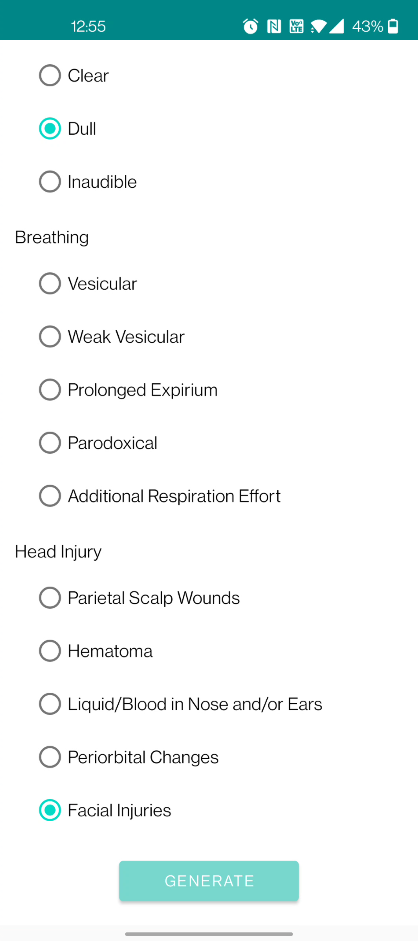
\includegraphics[width=0.4\textwidth]{figures/generate_report_screen.png}
\caption{The Generate Report Screen}
\label{fig:generate-report-screen}
\end{figure}

At the moment of writing this thesis the options for a report consist from some well defined Radio Buttons organized in Radio Groups based on the enum class they are part of. All of the available options can be seen in figure \ref{fig:report-options-diagram}.

\begin{figure}
\centering
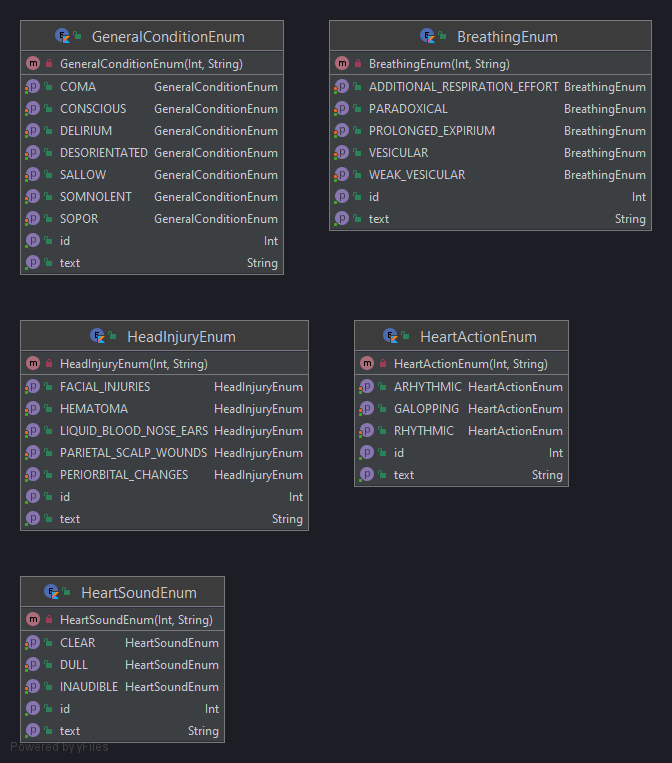
\includegraphics[width=0.75\textwidth]{figures/report_options_class_diagram.png}
\caption{Report Options Class Diagram}
\label{fig:report-options-diagram}
\end{figure}
\chapter{Potential future improvements}
\label{ch:6}

\par When looking back at the Medical Reports application we managed to create in order to implement the usage of NFC tags in a health care environment we can clearly see some of the improvements that are definitely needed in the future in order for this to be a viable solution.

First of all we need a better design. As straight forward as plain text is in order to communicate the information it is no better than a piece of paper. The application is not very appealing to the end user in its current state, with the exception of some screens.

A second area where we definitely see the place for an improvement is the user registration system. There needs to be a way to notify the users that their account was successfully confirmed, a role has been assigned and that they are able to now login in the mobile application. Perhaps a confirmation email would suffice.

When it comes to the way we are registering patients there should also be an improvement, as at this point we are only allowing the nurse to register a new patient, but not search for the patient in case it already exists and only assign a bracelet instead. In order to achieve this we would need to also collect, at the time of the registration, the social security number of the patient in order to uniquely identify him or her.

As stated in the subsection \ref{sec:ch2sec5subsec3}, in order to preserve the privacy of the data seen on devices we could also add a password or biometric locking mechanism before retrieving the information about a patient from the server in order to once again confirm the fact that the person operating the device is the authorized person, and not someone whom illegally got access to the authorized mobile device. Also we could add special security flags in order to restrict screenshots and screen recordings from the screens that contain sensitive information about the patient.

When it comes to the patients we think an option should be available to retrieve the information without the need of an NFC tag in order to maybe analyze the latest reports, or see in which room the patient is currently located in the hospital.

The reports are surely incomplete as there are many other options that should be available for a medical professional to complete as well as maybe some text fields they can freely complete (like some notes). Also when talking about the reports there should be a way to edit them later (as the author) and they should contain some timestamps that reflect the creation date and the latest update date.

Another improvement we see necessary is the possibility to generate different types of reports, for example a blood test results report that contains different fields than the normal report. While we are still talking about reports a nice to have functionality for the future would be for you to have a small unread icon next to the unread reports in order to notify the medical personnel that there are new reports that have been generated for that patient.

We can also see the possibility of an improvement by adding a settings screen where a profile view would be available for the user as well as a change password option and the Sign Out button.

We know that our solution is not yet complete, however we believe it is good enough at exemplifying what can be done using the NFC tags in order to safely and easily retrieve patient information from an EMR system.

\chapter{Conclusions}
\label{conclusions}

\par When talking about privacy and security, considering the improvements we have mentioned in chapter \ref{ch:6}, it is important that we learn the fact that no system can be completely secure and completely protected from prying eyes. A person which roots their device can easily bypass any flags that restricts screenshots and screen recordings as well as a biometric authentication in order to confirm their identity. However in those cases the biometric system can help making the data extraction harder giving enough time in some cases for the device to be either wiped or recovered.

However we will only be able to use the implementation we provided, as amazing as it is, in a restricted way. The reason behind our statement is that in order to take full advantage of it, a centralized system for all the health care institutes in a country would be necessary in order for all the necessary reports to be available when checking a patient's profile. We wish that this was not true, but centralizing all of the data in one big database presents a totally different security concern.

Keeping this in mind however, we still think there is potential for the NFC technology to be introduced in hospitals and medical institutes, even if in a much smaller scale, like a city for example. The benefits and the steps we could take forward using this approach in order to preserve the patient's privacy are worth the trouble.

To sum up everything that has been stated so far, we do believe that our solution, the "Medical Records" application, is an appropriate solution, and once improved with the features that we mentioned in chapter \ref{ch:6} could be modified to work with the existing EMR systems and used in order to meet the current standards regarding the privacy in the European Union.
%\addcontentsline{toc}{chapter}{Conclusions}

\bibliography{references}

\end{document}
